 %%%%%%%%%%%%%%%%%%%%%%%%%%%%%%%%%%%%%%%%%%%%%%%%%%%%%%%%%%%%%%%%%%%%%%%%%%%%%
%	e-Yantra, IIT-Bombay

%	Document Author: Akshit Gandhi
%	Date: 7-June,2016
%	Last Editted by: Akshit
%   Date Last updated: 6-07-2016 

%%%%%%%%%%%%%%%%%%%%%%%%%%%%%%%%%%%%%%%%%%%%%%%%%%%%%%%%%%%%%%%%%%%%%%%%%%%%%

\documentclass[11pt,a4paper]{article}
\usepackage{float}
\usepackage{graphicx}
\usepackage{hyperref}
\title{Assembling The Quadcopter}
\author{Keyur Rakholiya \\ Akshit Gandhi}
\date{\today}

\begin{document}
	\maketitle
	\newpage
	\tableofcontents
	\newpage
	\section{Objective}
	Topic: Assembling the quadcopter
		In this tutorial we will study about the assembling of the quadcopter.
	\section{Prerequisites}
	refer the previous tutorial first.
	1. calculation
	
	choose your flight controller, motors,propellers,frame,battery.
	\section{Hardware Requirement}
	 All the components mentioned previously and a Soldering kit, deans connector and wires, M3*8 screws.
	\section{Assembly}
	 So, now we start with the assembly of the quad, ensure you have all the components mentioned previously.
	 \subsection{Assembling the Motors}
	 	Once you get the motors, the very first job is to mount the motors on the F450 frame. For this you will need M3 screws, so with the help of a screw-driver or L-key mount the motors on the arm of the quad like this:
	 	\begin{figure}[h]
	 	
	 	\centering
		\includegraphics[width=5cm,height=5cm]{screw}
		\caption{installing motors}
	 	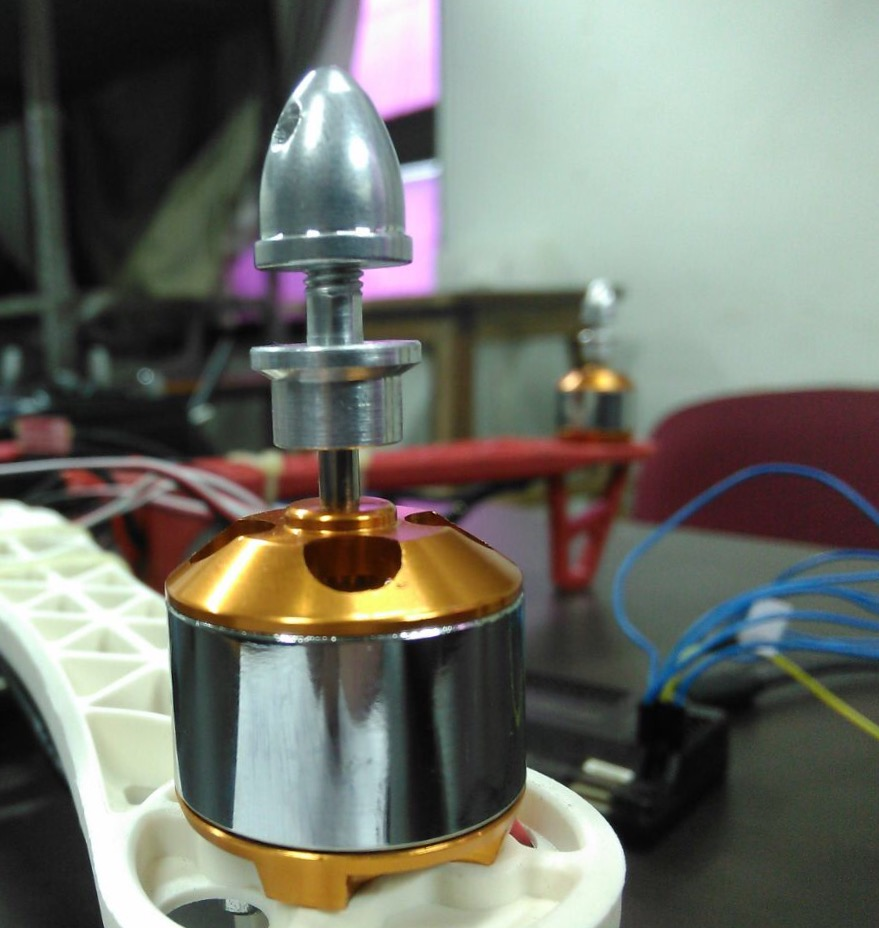
\includegraphics[width=5cm,height=5cm]{mot}
	 	\caption{Motor Assembly.}
\end{figure}
	 	\subsection{Esc mount}
	 	After the motors have been attached on the arms, next job is to attach the esc's, you can tie individual esc's on the arms using cable ties as shown below.
		 	
	 	 Also connect 3 wires from the esc's to the 3 wires on the motor, don't worry about the order in which the wires have to be connected we will look upon that in later tutorials.on ce your arms are ready with the escs and motors it will look something like this:
	 	 \begin{figure}[h]
	 	
	 	\centering
		\includegraphics[width=10cm,height=5cm]{esc}
		\caption{Esc Assembly.}
		\end{figure}
		
		\subsection{Connecting Esc to Power distribution board}
		The F450 frame comes with an inbuilt power distribution board so you just need to solder the esc wires (both positive and ground) to the pcb on the base plate. The pcb would look something like this.
		\begin{figure}[h]
	 	
	 	\centering
		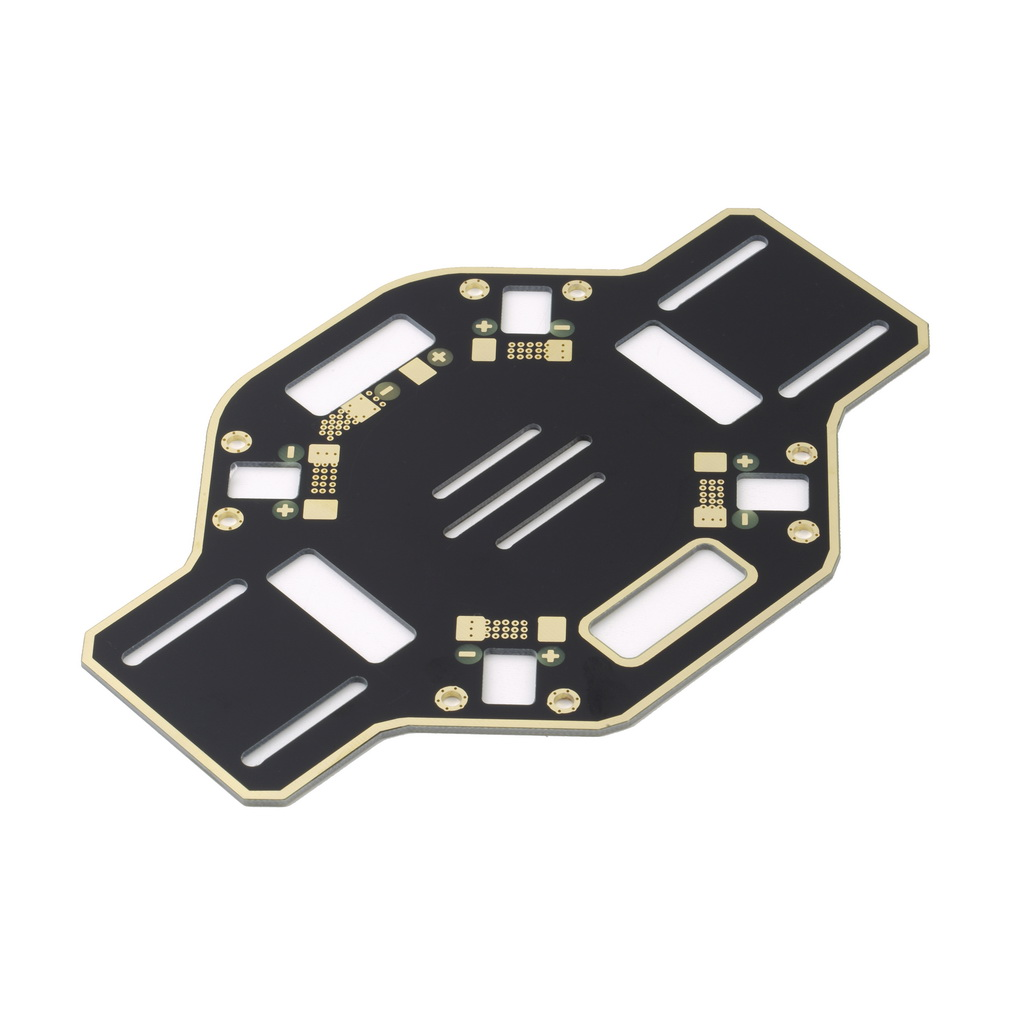
\includegraphics[width=7cm,height=7cm]{pcb}
		\caption{Power distribution Board.}
		\end{figure}
		
You will see that there are some points to attach the esc's marked as + or - and also on extra pair of points will be there for connecting the battery to the distribution board. First you need to ensure that there are no connectors on the esc( on the +ve and -ve wires), if there are any connectors desolder them and then solder the wires onto the pcb. Special care to ensure that +ve wires is soldered onto the +ve of the pcb and respectively for negative. Once you have soldered the wires onto the assembly would look something like this:
		\begin{figure}[h]
	 	
	 	\centering
		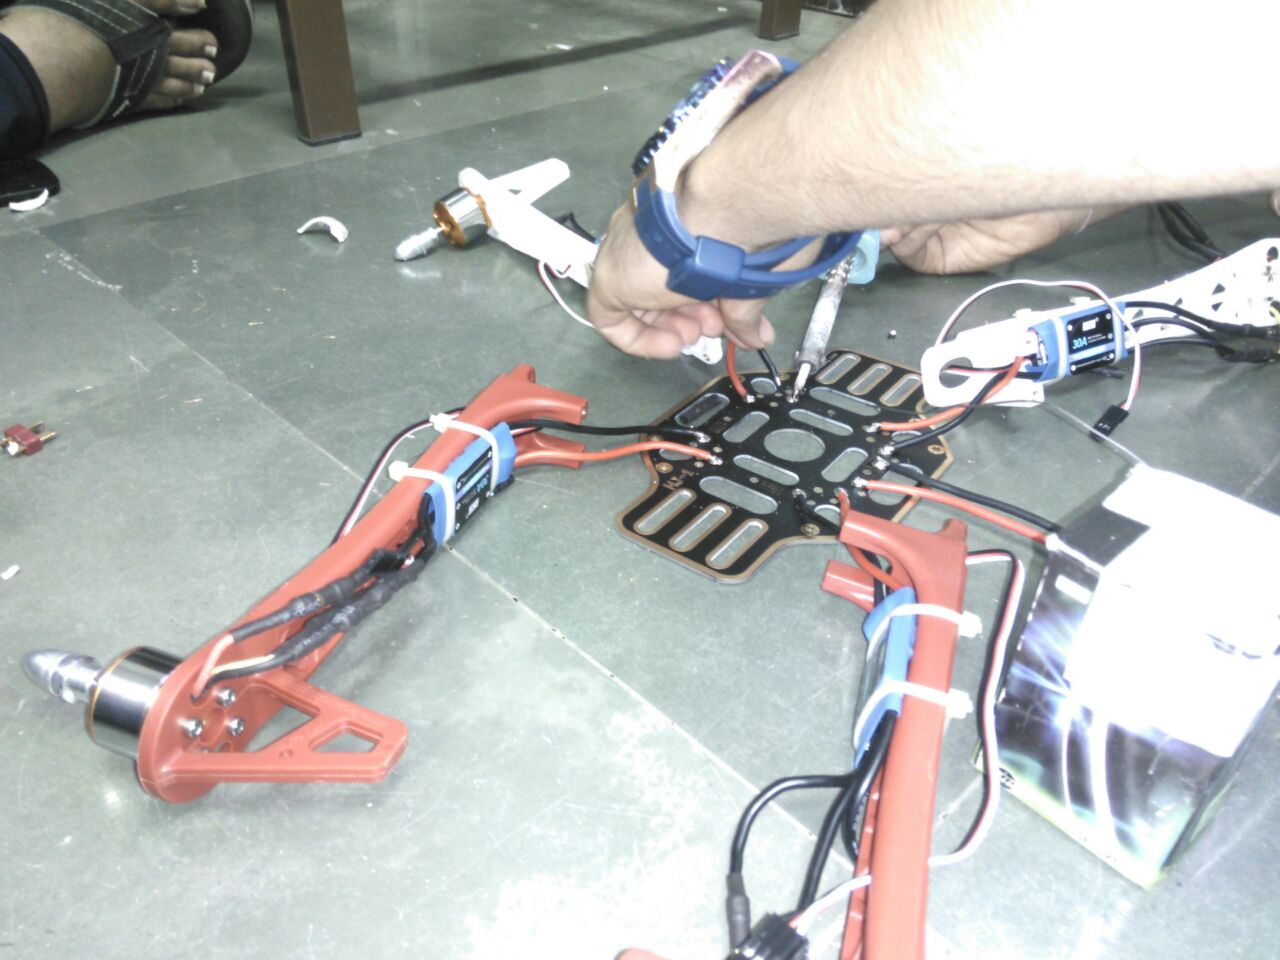
\includegraphics[width=12cm,height=6.5cm]{solder}
		\caption{Soldering.}
		\end{figure}
		
		\begin{figure}[h]
	 	
	 	\centering
		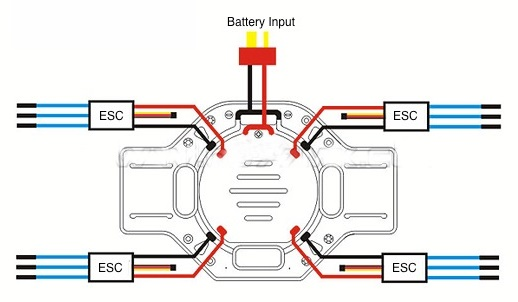
\includegraphics[width=12cm,height=6.5cm]{wiring}
		\caption{Wiring Schematic.}
		\end{figure}
		
		\subsection{Putting the frame together}
		Now you have your frame ready the next step is to use the screws provided with the kit to mount the arms on the lower plate and after that attach the upper plate. After this step your quad should look like this:
		\paragraph{}But an IMPORTANT note: To make it easy for you to know the orientation of the quad you can setup the frame in such a way that 2 adjacent white/red arms point to the forward direction of the quad.
		\begin{figure}[h]
	 	
	 	\centering
		\includegraphics[width=12cm,height=7cm]{frame}
		\caption{Frame Assembly w/o upper plate mounted.}
		\end{figure}
		
		\subsection{Mounting your Flight Controller}
		For the autonomous drone application we are usin APM 2.6 as our flight controller, but you can use any flight controller of your choice like KK 2.x board, CC3D, Naze 32, Pixhawk, KISS,etc. The basic step to mount any flight controller on the deck of the frame is by mounting it by using an anti-vibration mount. Using it is very important as it reduces the amount of vibrations that reach the controller. As unwanted vibrations can lead to erroneous results.
		\paragraph{}So were are using the antivibration mount for the APM. So depending on your flight controller you can mount it on the mount by using double sided tapes. But before mounting the vibration mount on the deck ensure that the forward direction of the FC matches with the forward direction of your quad decided by you.
		
		\subsection{Wiring the flight controller}
		Now depending on your flight controller you have to wire up your Flight controller with the receiver and the ESC's. Here we will demonstrate the connections for the APM 2.6 .
		\paragraph{} Another important note is to make the motor connections properly i.e. the first motor connects to port 1 on the APM and son on. The below pictures will make it very clear.
		\begin{figure}[h]
	 	\centering
		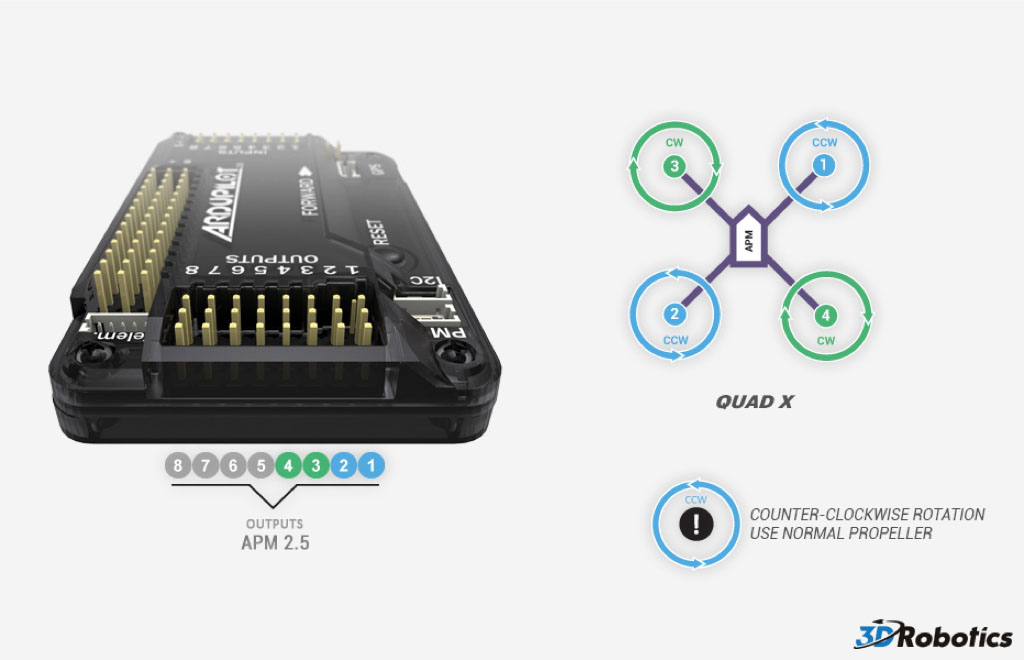
\includegraphics[width=12cm,height=7cm]{direction}
		\caption{Motor Layout For quad X config.}
		\end{figure}
		\paragraph{}Don't worry about the motor spin direction we will solve it in a moment. Now let's see how to make connections with the APM. Refer the below figure. Don't bother about the GPS and Gimbal, they are just extra accessories.
		\begin{figure}[H]
    \begin{center}
    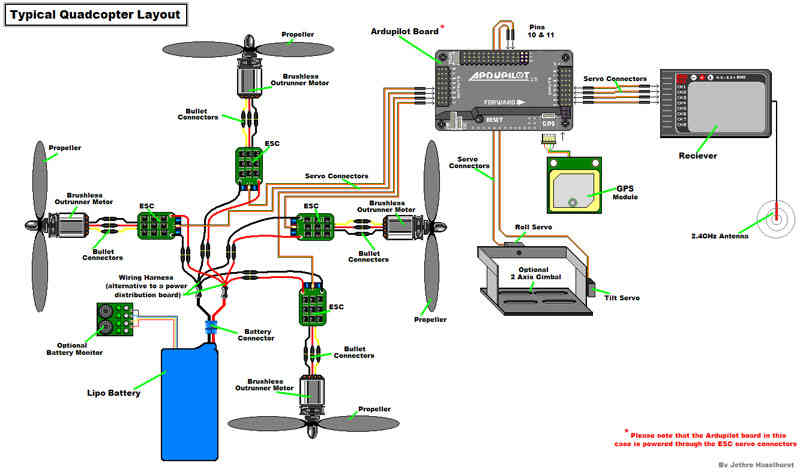
\includegraphics[scale=0.6]{APM}
    \caption{APM wiring}
    \label{fig: figure}
    \end{center}
\end{figure}
	\paragraph{•}
	Now if you have followed the above steps properly, you are ready for the calibration of your flight controller. Now here we are done with the assembly.
	\section{References}
	Images are downloaded from:
	\paragraph{•}
	\url{http://ardupilot.org/copter/docs/connecting-the-apm2.html}
	\paragraph{•}\url{https://multicopterbuild.wordpress.com/how-tos/quadcopter/}
	\paragraph{•}\url{http://dronesforsaleclassified.com/product/dji-hot-wheels-diy-same-paragraph-quadcopter-frame-quality-nylon-f450-v2-rack-integrated-pcb-board-diy-drone-quadrocopter/}
	\paragraph{•}\url{http://www.flyingtech.co.uk/frames-props-parts-accessories/tarot-firefly-450-quadcopter-frame}
	
\end{document}



